\begin{frame}{Montgomery Ladder}
    \begin{definitionblock}{Montgomery Ladder}
        \\Algorithmus zur Skalarmultiplikation auf Montgomery-Kurven:
        \begin{itemize}
            \item Berechnung nur mit $x$-Koordinaten
            \item Konstante Laufzeit
        \end{itemize}
    \end{definitionblock}
    \vspace{2em}
    \[\textbf{x}:\mathcal{E}\rightarrow \mathcal{E}/\langle\ominus\rangle=\mathbb{P}^1\]
    \begin{align*}
    \textbf{x}: P \longmapsto
    \begin{cases}
        (X_P:1) & \text{für } P = (X_P:Y_P:1), \\
        (1:0) & \text{für } P = \mathcal{O} = (0:1:0).
    \end{cases}
\end{align*}
\end{frame}
\begin{frame}{Montgomery Ladder}
   
        
        
            \begin{definitionblock}{Pseudo-Operationen}
                \vspace{-1em}
                \begin{align*}
                    \texttt{xDBL:}&\textbf{x}(P)\longmapsto \textbf{x}([2]P) \\
                    \texttt{xADD:}&(\textbf{x}(P),\textbf{x}(Q),\textbf{x}(P\ominus Q))\longmapsto \textbf{x}(P\oplus Q)
                \end{align*}
                
            \end{definitionblock}
            \begin{center}
               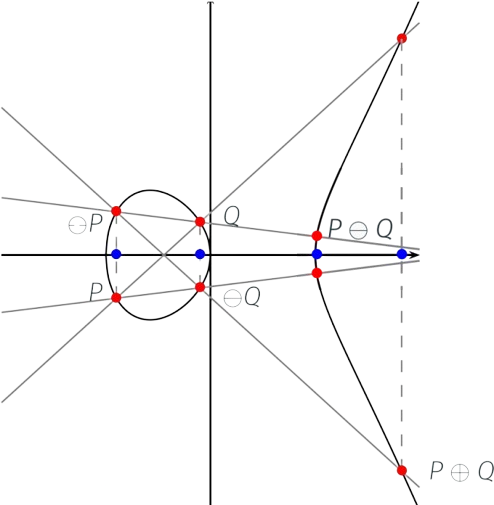
\includegraphics[width=0.35\linewidth]{img/x_cor} 
            \end{center}
       
\end{frame}
\begin{frame}{Montgomery Ladder}
    \begin{columns}
    \begin{column}{0.5\textwidth}
        \textbf{\texttt{xDBL}}\\
    \vspace{-1.8em}
    \begin{align*}
        x_{[2]P}&=B\lambda^2-2x_P-A\\
        &=\frac{(3x_P+2Ax_P+1)^2}{4By^2_P}\\&\quad-2x_P-A\\
        &=\frac{(x_P^2-1)^2}{4(x_P^3+Ax_P^2+x_P)}
    \end{align*}
    \end{column}
    \begin{column}{0.5\linewidth}
    \begin{align*}
        \textbf{\texttt{xADD}}\\
        &x_{P\oplus Q} x_{P\ominus Q}\\
        &= \left(B\left(\frac{(y_Q - y_P)^2}{(x_Q - x_P)^2}\right)  - (x_P + x_Q)-A\right)\\
        &\quad\cdot\left(B\left(\frac{(-y_Q - y_P)^2}{(x_Q - x_P)^2}\right)  - (x_P + x_Q)-A\right)\\
        &=  \frac{(x_Qx_P-1)^2}{(x_Q-x_P)^2}
    \end{align*}
    \end{column}
        
    \end{columns}
    \begin{itemize}
        \item Inversionen sind in endlichen Körpern rechenintensiv
        \item Projektive Koordinaten vermeiden direkte Inversion
        \item Darstellung der $x$-Koordinate als Bruch $\frac{X}{Z}$
        \item Rückwandlung in die affine Koordinate durch $x=XZ^{p-2}$
    \end{itemize}
    
\end{frame}

\begin{frame}{Montgomery Ladder}
    \begin{algorithmblock}
    \textbf{Notation}\\
    \vspace{-1.5em}
    \begin{center}
        $(X_P:Z_P)\coloneqq\textbf{x}(P),$ \quad $(X_Q:Z_Q)\coloneqq\textbf{x}(Q)$ \\
        \vspace{1em}
        $(X_\oplus:Z_\oplus)\coloneqq\textbf{x}(P\oplus Q),$ \quad $(X_\ominus:Z_\ominus)\coloneqq\textbf{x}(P\ominus Q)$
    \end{center}
    \end{algorithmblock}
    \vspace{1em}
    \begin{columns}
        \begin{column}{0.5\textwidth}
            \textbf{\texttt{xDBL}}
            \begin{align*}
                X_{[2]P} &= (X_P^2-Z_P^2)^2 \\
                Z_{[2]P} &= 4X_PZ_P(X_P^2+AX_PZ_P+Z_P^2)
\end{align*}
            
        \end{column}
        \begin{column}{0.5\textwidth}
            \textbf{\texttt{xADD}}
            \begin{align*}
                X_{\oplus} &= 4(X_PX_Q-Z_PZ_Q)Z_{\ominus} \\
                Z_{\oplus} &= 4(X_PZ_Q - Z_PX_Q)X_\ominus
            \end{align*}
        \end{column}
    \end{columns}
\end{frame}

\begin{frame}{Montgomery Ladder}
    \begin{columns}
        \begin{column}{0.4\textwidth}
            \textbf{\texttt{xDBL}}
            \begin{align*}
                X_{[2]P} &= (X_P + Z_P)^2 (X_P - Z_P)^2 \\
                Z_{[2]P} &= (4X_PZ_P)((X_P - Z_P)^2 \\ &\quad+ \left((A + 2)/4)(4X_PZ_P)\right)
\end{align*} \\
\textbf{\texttt{xADD}}
            \begin{align*}
                X_{\oplus} &= Z_{\ominus} [ (X_P - Z_P)(X_Q + Z_Q) \\
                & \quad + (X_P + Z_P)(X_Q - Z_Q) ]^2 \\
                Z_{\oplus} &= X_{\ominus} [ (X_P - Z_P)(X_Q + Z_Q) \\
                &\quad - (X_P + Z_P)(X_Q - Z_Q) ]^2
                \end{align*}
            
        \end{column}
        \begin{column}{0.7\textwidth}
            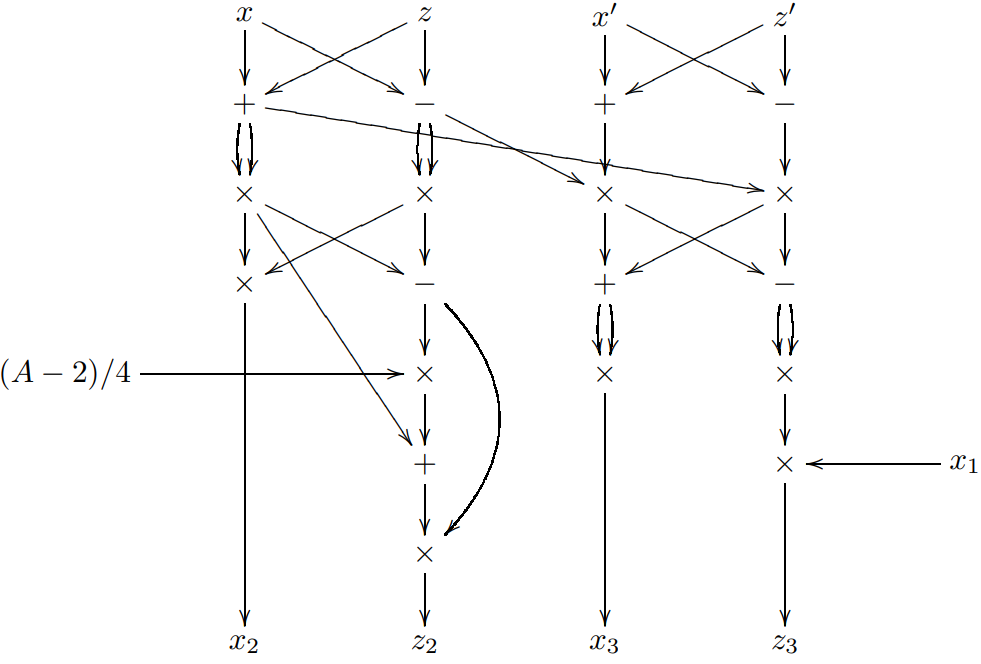
\includegraphics[width=1\textwidth]{tex/img/ladder.png}
      
        \end{column}
    \end{columns}
    
\end{frame}

\begin{frame}{Montgomery Ladder}
    \begin{algorithm}[H]
        \caption{\textbf{Algorithmus: Montgomery Ladder}}
        
        
        \textbf{Input:} $(1)\ k=\sum\nolimits_{i=0}^{l-1}k_i2^i$ mit $k_{l-1}=1$ \hfill \texttt{//Binärdarstellung des Skalars} \\ 
        \text{} $\quad \quad \quad \; (2)\ (X_P,Z_P)$, so dass $(X_P:Z_P)=\textbf{x}(P)$ \\
        \textbf{Output:} $(X_k,Z_k)$, so dass $(X_k:Z_k)=\textbf{x}([k]P)$
        
        \begin{algorithmic}[1]
            \State $\texttt{(x$_0$,x$_1$)} \gets ((X_P, Z_P), \texttt{xDBL}(X_P, Z_P))$ \hfill \texttt{//x$_1$-x$_0$ ist immer $(X_P,Z_P)$} \\
            \textbf{for} $i = l-2$ \textbf{downto} 0 \textbf{do}\\
            \quad \textbf{if} $k_i = 0$ \textbf{then}
            \State \quad \quad $\texttt{(x$_0$,x$_1$)} \gets (\texttt{xDBL}(\texttt{x$_0$}),\texttt{xADD}(\texttt{x$_0$},\texttt{x$_1$},(X_P,Z_P)))$ \\
            \quad \textbf{else}
            \State \quad \quad $\texttt{(x$_0$,x$_1$)} \gets (\texttt{xADD}(\texttt{x$_0$},\texttt{x$_1$},(X_P,Z_P)),\texttt{xDBL}(\texttt{x$_1$}))$
            \State \textbf{return} $\texttt{x$_0$}$ \hfill \texttt{//x$_0$}$=\textbf{x}([k]P)$, \texttt{x$_0$}$=\textbf{x}([k+1]P)$
            
         
        \end{algorithmic}
    \end{algorithm}
    
\end{frame}

